\section{Przykład działania}

\tikzset{
  every node/.style={circle,fill=black!40},
  0/.style={fill=red!50},
  1/.style={fill=purple!50},
  2/.style={fill=green!50},
  3/.style={fill=yellow!50},
  4/.style={fill=cyan!50},
  5/.style={fill=blue!50}
}

Poniżej przedstawiono przykładowy przebieg działania programu.

Dane wejściowe:

\begin{itemize}
  \item Graf:

    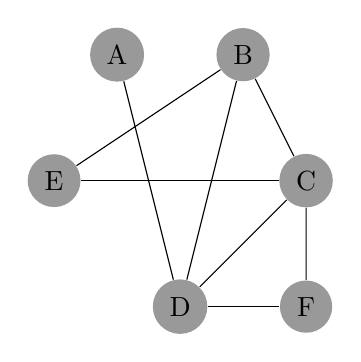
\begin{tikzpicture}[scale=.8]
      \node (A) at (2,4) {A};
      \node (B) at (4,4) {B};
      \node (C) at (5,2) {C};
      \node (D) at (3,0) {D};
      \node (E) at (1,2) {E};
      \node (F) at (5,0) {F};

      \foreach \from/\to in {A/D,B/C,B/D,B/E,C/D,C/E,C/F,D/F}
        \draw (\from) -- (\to);
    \end{tikzpicture}

  \item Zestaw kolorów:
    
\begin{tikzpicture}[scale=.8]
      \node [0] (A) at (0,0) {};
      \node [1] (B) at (0.5,0) {};
      \node [2] (C) at (1,0) {};
      \node [3] (D) at (1.5,0) {};
      \node [4] (E) at (2,0) {};
      \node [5] (F) at (2.5,0) {};
    \end{tikzpicture}
    
  \item Wielkość pmięci: $3$
  
  \item Maksymalna liczba iteracji: $100$
  
  \item Maksymalna liczba iteracji bez zmiany rezultatu: $2$
\end{itemize}

Przykładowy wynik:

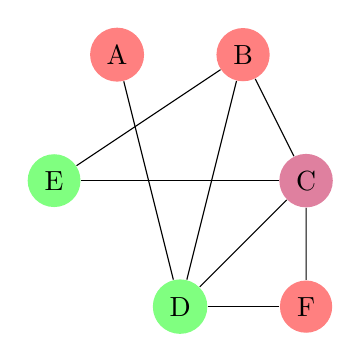
\begin{tikzpicture}[scale=.8]
  \node [0] (A) at (2,4) {A};
  \node [0] (B) at (4,4) {B};
  \node [1] (C) at (5,2) {C};
  \node [2] (D) at (3,0) {D};
  \node [2] (E) at (1,2) {E};
  \node [0] (F) at (5,0) {F};

  \foreach \from/\to in {A/D,B/C,B/D,B/E,C/D,C/E,C/F,D/F}
    \draw (\from) -- (\to);
\end{tikzpicture}



\subsection{Przygotowanie grafu} \label{sec:exmpl_graph_prep}
Przed rozpączęciem właściwego działania algorytmu, program buduje graf~i dokonuje jego losowego pokolorowania.

\begin{itemize}
  \item Graf:

    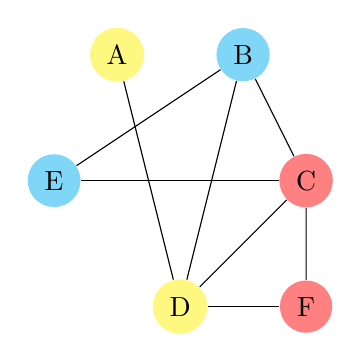
\begin{tikzpicture}[scale=.8]
      \node [3] (A) at (2,4) {A};
      \node [4] (B) at (4,4) {B};
      \node [0] (C) at (5,2) {C};
      \node [3] (D) at (3,0) {D};
      \node [4] (E) at (1,2) {E};
      \node [0] (F) at (5,0) {F};

      \foreach \from/\to in {A/D,B/C,B/D,B/E,C/D,C/E,C/F,D/F}
        \draw (\from) -- (\to);
    \end{tikzpicture}

  \item Lista tabu: pusta
\end{itemize}


\subsection{Przeszukiwanie}
W każdym kroku algorytm sprawdza wszystkich sąsiadów aktualnego grafu.
Jako aktualny graf obiera tego sąsiada, dla którego wartość funkcji celu jest najmniejsza.

\subsubsection{Krok 1}
\begin{itemize}
  \item Akcja:
   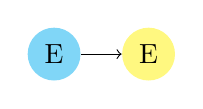
\begin{tikzpicture}[->,scale=.8]
     \node [4] (1) at (0,0) {E};
     \node [3] (2) at (1.5,0) {E};

     \foreach \from/\to in {1/2}
       \draw (\from) -> (\to);
   \end{tikzpicture}

  \item Wartość funkcji celu: $-4$

  \item Graf:

    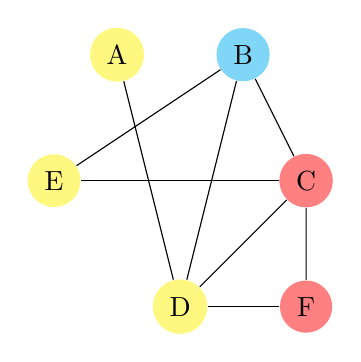
\begin{tikzpicture}[scale=.8]
      \node [3] (A) at (2,4) {A};
      \node [4] (B) at (4,4) {B};
      \node [0] (C) at (5,2) {C};
      \node [3] (D) at (3,0) {D};
      \node [3] (E) at (1,2) {E};
      \node [0] (F) at (5,0) {F};

      \foreach \from/\to in {A/D,B/C,B/D,B/E,C/D,C/E,C/F,D/F}
        \draw (\from) -- (\to);
    \end{tikzpicture}

  \item Lista tabu:
    
\begin{tikzpicture}[scale=.8]
      \node [4] (E) at (0,0) {E};
    \end{tikzpicture}
\end{itemize}


\subsubsection{Krok 2}

\begin{itemize}
  \item Akcja:
   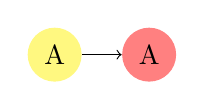
\begin{tikzpicture}[->,scale=.8]
     \node [3] (1) at (0,0) {A};
     \node [0] (2) at (1.5,0) {A};

     \foreach \from/\to in {1/2}
       \draw (\from) -> (\to);
   \end{tikzpicture}

  \item Wartość funkcji celu: $-8$

  \item Graf:

    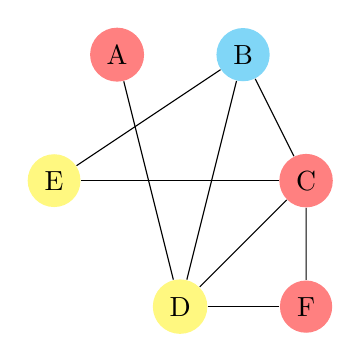
\begin{tikzpicture}[scale=.8]
      \node [0] (A) at (2,4) {A};
      \node [4] (B) at (4,4) {B};
      \node [0] (C) at (5,2) {C};
      \node [3] (D) at (3,0) {D};
      \node [3] (E) at (1,2) {E};
      \node [0] (F) at (5,0) {F};

      \foreach \from/\to in {A/D,B/C,B/D,B/E,C/D,C/E,C/F,D/F}
        \draw (\from) -- (\to);
    \end{tikzpicture}

  \item Lista tabu:
    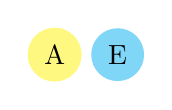
\begin{tikzpicture}[scale=.8]
      \node [3] (A) at (-1,0) {A};
      \node [4] (E) at (0,0) {E};
    \end{tikzpicture}
\end{itemize}


\subsubsection{Krok 3}

\begin{itemize}
  \item Akcja:
   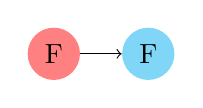
\begin{tikzpicture}[->,scale=.8]
     \node [0] (1) at (0,0) {F};
     \node [4] (2) at (1.5,0) {F};

     \foreach \from/\to in {1/2}
       \draw (\from) -> (\to);
   \end{tikzpicture}

  \item Wartość funkcji celu: $-12$

  \item Graf:

    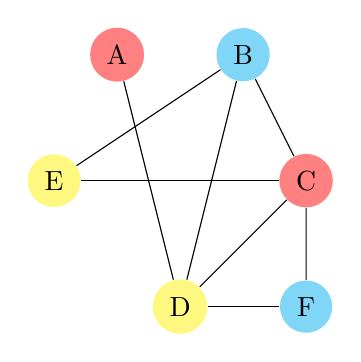
\begin{tikzpicture}[scale=.8]
      \node [0] (A) at (2,4) {A};
      \node [4] (B) at (4,4) {B};
      \node [0] (C) at (5,2) {C};
      \node [3] (D) at (3,0) {D};
      \node [3] (E) at (1,2) {E};
      \node [4] (F) at (5,0) {F};

      \foreach \from/\to in {A/D,B/C,B/D,B/E,C/D,C/E,C/F,D/F}
        \draw (\from) -- (\to);
    \end{tikzpicture}

  \item Lista tabu:
    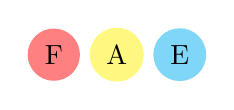
\begin{tikzpicture}[scale=.8]
      \node [0] (F) at (-2,0) {F};
      \node [3] (A) at (-1,0) {A};
      \node [4] (E) at (0,0) {E};
    \end{tikzpicture}
\end{itemize}


\subsubsection{Krok 4}

\begin{itemize}
  \item Akcja:
   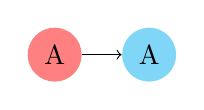
\begin{tikzpicture}[->,scale=.8]
     \node [0] (1) at (0,0) {A};
     \node [4] (2) at (1.5,0) {A};

     \foreach \from/\to in {1/2}
       \draw (\from) -> (\to);
   \end{tikzpicture}

  \item Wartość funkcji celu: $-14$

  \item Graf:

    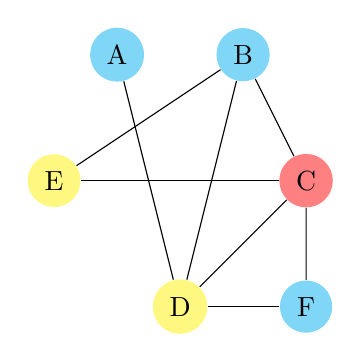
\begin{tikzpicture}[scale=.8]
      \node [4] (A) at (2,4) {A};
      \node [4] (B) at (4,4) {B};
      \node [0] (C) at (5,2) {C};
      \node [3] (D) at (3,0) {D};
      \node [3] (E) at (1,2) {E};
      \node [4] (F) at (5,0) {F};

      \foreach \from/\to in {A/D,B/C,B/D,B/E,C/D,C/E,C/F,D/F}
        \draw (\from) -- (\to);
    \end{tikzpicture}

  \item Lista tabu:
    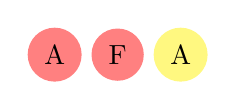
\begin{tikzpicture}[scale=.8]
      \node [0] (A) at (-2,0) {A};
      \node [0] (F) at (-1,0) {F};
      \node [3] (A) at (0,0) {A};
    \end{tikzpicture}
\end{itemize}

W tym momencie znalezione zostało optymalne pokolorowanie grafu.
Program nie sprawdza jednak poprawności pokolorowania w każdym kroku, dlatego kontynuuje działanie.


\subsubsection{Krok 5}

\begin{itemize}
  \item Akcja:
   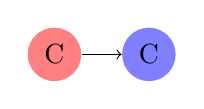
\begin{tikzpicture}[->,scale=.8]
     \node [0] (1) at (0,0) {C};
     \node [5] (2) at (1.5,0) {C};

     \foreach \from/\to in {1/2}
       \draw (\from) -> (\to);
   \end{tikzpicture}

  \item Wartość funkcji celu: $-14$

  \item Graf:

    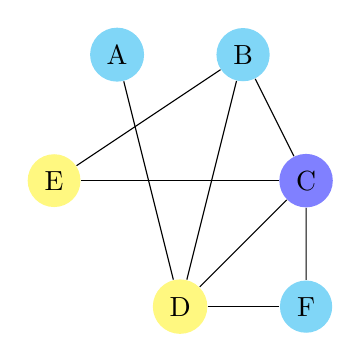
\begin{tikzpicture}[scale=.8]
      \node [4] (A) at (2,4) {A};
      \node [4] (B) at (4,4) {B};
      \node [5] (C) at (5,2) {C};
      \node [3] (D) at (3,0) {D};
      \node [3] (E) at (1,2) {E};
      \node [4] (F) at (5,0) {F};

      \foreach \from/\to in {A/D,B/C,B/D,B/E,C/D,C/E,C/F,D/F}
        \draw (\from) -- (\to);
    \end{tikzpicture}

  \item Lista tabu:
    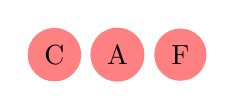
\begin{tikzpicture}[scale=.8]
      \node [0] (C) at (-2,0) {C};
      \node [0] (A) at (-1,0) {A};
      \node [0] (F) at (0,0) {F};
    \end{tikzpicture}
\end{itemize}

W tym momencie osiągnięto maksymalną liczbę iteracji bez zmiany rezultatu.
Program kończy działanie, jako wynik podając graf otrzymany w kroku 4 (jako że graf otrzymany w kroku 5 nie jest od niego lepszy).